\thispagestyle{empty}
\newgeometry{top=4cm, bottom=4cm, left=4cm, right=4cm} 

\setlength{\parindent}{2em}
\setlength{\parskip}{0em}
\setlength{\columnsep}{2em}

\begin{multicols}{2}
\noindent
При схождении в одной вершине двух многоугольников у одного из них внутренний угол должен быть более $2d (180^{\circ})$. что, очевидно, также невозможно. Таким образом, решение задачи распадается на анализ тех вариантов, когда в вершине паркета сходятся 3, 4, 5 и 6 правильныл многоугольников.
\\[3em]
\noindent
\textbf{Паркеты с тремя многоугольниками в вершине}\\
Здесь, в свою очередь, в принципе возможны три случая (в зависимости от набора многоугольников в каждой вершине):

\begin{compactitem}
  \item [$1^{\circ}$] Три одинаковых многоугольника.
  \item [$2^{\circ}$] Два одинаковых и один отличный от них.
  \item [$3^{\circ}$] Три различных многоугольника.
\end{compactitem}

В \textit{первом случае} сумма в уравнении (1) сводится к одному слагаемому, отвечающему трем одинаковым п-угольникам, поэтому мы\linebreak получаем $3(1-\frac{2}{n})=2$ или $n=6$,\linebreak
то есть к каждой вершине примыкает $3$ шестиугольника. Это один из простейших правильных паркетов (рис. 1)

Для \textit{второго случая} (два $k$ - угольника, один $n$-угольник) имеем \linebreak
$(1-\frac{2}{n})+2(1-\frac{2}{k})=2$ или $k=\frac{4n}{n-2}$.\linebreak
Целочисленные решения последнего уравнения проще всего найти перебором различных значений:

\vspace{2em}
\noindent
\resizebox{\columnwidth}{!}{
\begin{tabular}{ c|c c c c c c c c c c c } 

    n & 1 & 2 & 3 & 4 & 5 & 6 & 7 & 8 & 9 & 10 & 11 \\ 
    \hline \\
    k & & & 12 & 8 & $\frac{20}{3}$ & 6 & $\frac{28}{5}$ & $\frac{32}{6}$ & $\frac{36}{7}$ & 5 & $\frac{44}{9}$
\end{tabular}}

\vspace{1em}
\noindent
Продолжать перебор дальше нет смысла, так как целочисленных $k$ мы больше не получим:
$\frac{4n}{n-2}=4+\frac{8}{n-2}$,\linebreak
а при $n>10$ последнее слагаемое не может быть целым.

Таким образом, кроме уже рассмотренного случая $n=k=6$ мы получили три решения, которые мы запишем в виде суммы углов в 

\columnbreak 
\begin{Figure}
    \centering
    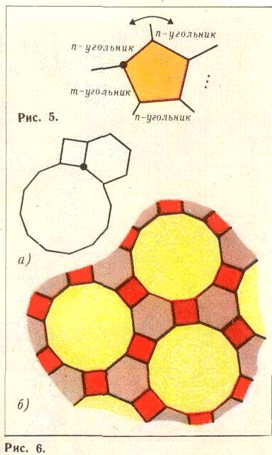
\includegraphics[width=\columnwidth]{pic_1}
\end{Figure}


\noindent
вершине:
$\alpha_4 + 2\alpha_8$; \ $\alpha_3+2\alpha_1_2$; \ $\alpha_1_0+2\alpha_5$.

Первому решению отвечает паркет, часто встречающийся на практике (рис. 2), Менее обычный паркет, отвечающий второму решению, изображен на рисунке 3.

А вот комбинация $\alpha_1_0 + 2\alpha_5$, в
отличие от ранее рассмотренных, правильного паркета не образует. Убедиться в этом позволяет «достройка» (рис. 4) окружения вершины $А$ еще одним многоугольником (желтого цвета). Из нее видно, что один из углов при вершине $В$ (угол, обозначенный на рисунке 4 через $\phi$ по принципу эквивалентности вершин, должен быть равен $\alpha_1_0$. На самом же деле, угол $\phi$ равен $\alpha_5$ — правильного паркета типа $\alpha_1_0 + 2\alpha_5$ \textit{не существует}.

Для оставшегося, наиболее сложного, \textit{третьего случая} (три разных многоугольника с $n$, $m$ и $k$ вершинами) уравнение (1) приводится к виду
\begin{center}
    $\frac{1}{n} + \frac{1}{m} + \frac{1}{k} = \frac{1}{2}$. \ \ \ \ \ \ (2)
    
\end{center}
Чтобы не разбирать всех возможных
\vspace{\fill}
\begin{flushright}
    11
\end{flushright}
\end{multicols}

